\section{Reconstruction and Sparsity}\label{sec:recon}

Table~\ref{tab:recon} and Figure~\ref{fig:recon} (left) give OWT test reconstruction for all 108 SAEs
(\evlabel{test}). Explained variance falls with depth for every architecture, from 0.93--0.95 at layers 0--2 to
0.757 (ReLU) and 0.815 (TopK, JumpReLU) at layer 11. Among matched runs, ReLU leads at layer 1, ReLU and JumpReLU tie
at layer 2, JumpReLU leads at layers 3--9, and JumpReLU and TopK tie at layers 10--11. Seed standard deviations are
$\le 0.001$ except for layer-0 JumpReLU, whose seed 42 is unmatched (L0 73.6; about 96\,\% of latents dead) and
excluded from rankings.

\paragraph{Sparsity is matched on OWT only.} ReLU runs 2--6\,\% above the target L0. A within-layer adjustment using
the L0 elasticity measured in an earlier sweep changes no ranking except two near-ties (M0). The architectures differ
strongly in effective width: of 3072 latents, ReLU keeps 2920--3063 alive, TopK 1711--2851 and JumpReLU 469--2947. On
task prompts the number of active latents is not matched (on GoT final tokens, TopK uses 128, ReLU 32--110 and
JumpReLU 23--92 at layers 1--11), which confounds architecture comparisons on task information (\S\ref{sec:info}).

% generated by scripts/shared/build_paper_artifacts.py from results/openwebtext/reconstruction_evaluation/uninterrupted_protocol/all_layers_summary.csv
\begin{table}[t]
\centering
\small
\caption{Reconstruction on the OWT test split (TEST; 12{,}700 tokens), width 3072, target L0 = 128. Layer-0 JumpReLU includes the unmatched seed 42 (L0 73.6). Source: \texttt{results/\allowbreak{}openwebtext/\allowbreak{}reconstruction\_evaluation/\allowbreak{}uninterrupted\_protocol/\allowbreak{}all\_layers\_summary.csv}.}
\label{tab:recon}
\begin{adjustbox}{max width=\linewidth}
\begin{tabular}{rcccccc}
\toprule
Layer & \multicolumn{3}{c}{OWT test EV (mean$\pm$sd, 3 seeds)} & \multicolumn{3}{c}{OWT test L0} \\
\cmidrule(lr){2-4}\cmidrule(lr){5-7}
 & ReLU & TopK & JumpReLU & ReLU & TopK & JumpReLU \\
\midrule
0 & 0.950$\pm$0.000 & 0.911$\pm$0.000 & 0.826$\pm$0.101 & 135.1 & 125.3 & 110.3 \\
1 & 0.937$\pm$0.000 & 0.921$\pm$0.001 & 0.933$\pm$0.000 & 132.2 & 128.0 & 129.3 \\
2 & 0.936$\pm$0.000 & 0.926$\pm$0.000 & 0.935$\pm$0.002 & 131.9 & 128.0 & 129.0 \\
3 & 0.905$\pm$0.000 & 0.906$\pm$0.000 & 0.915$\pm$0.001 & 131.7 & 128.0 & 129.1 \\
4 & 0.872$\pm$0.000 & 0.884$\pm$0.000 & 0.893$\pm$0.001 & 131.1 & 128.0 & 129.1 \\
5 & 0.848$\pm$0.000 & 0.868$\pm$0.000 & 0.875$\pm$0.000 & 130.8 & 128.0 & 129.0 \\
6 & 0.832$\pm$0.001 & 0.857$\pm$0.000 & 0.865$\pm$0.000 & 131.0 & 128.0 & 129.1 \\
7 & 0.819$\pm$0.001 & 0.850$\pm$0.000 & 0.855$\pm$0.000 & 131.4 & 128.0 & 129.9 \\
8 & 0.805$\pm$0.000 & 0.840$\pm$0.000 & 0.844$\pm$0.000 & 131.9 & 128.0 & 130.3 \\
9 & 0.789$\pm$0.001 & 0.831$\pm$0.000 & 0.833$\pm$0.000 & 132.4 & 128.0 & 131.0 \\
10 & 0.773$\pm$0.000 & 0.822$\pm$0.000 & 0.823$\pm$0.000 & 132.7 & 128.0 & 131.6 \\
11 & 0.757$\pm$0.001 & 0.815$\pm$0.000 & 0.815$\pm$0.000 & 133.2 & 128.0 & 132.1 \\
\bottomrule
\end{tabular}
\end{adjustbox}
\end{table}


\begin{figure}[t]
  \centering
  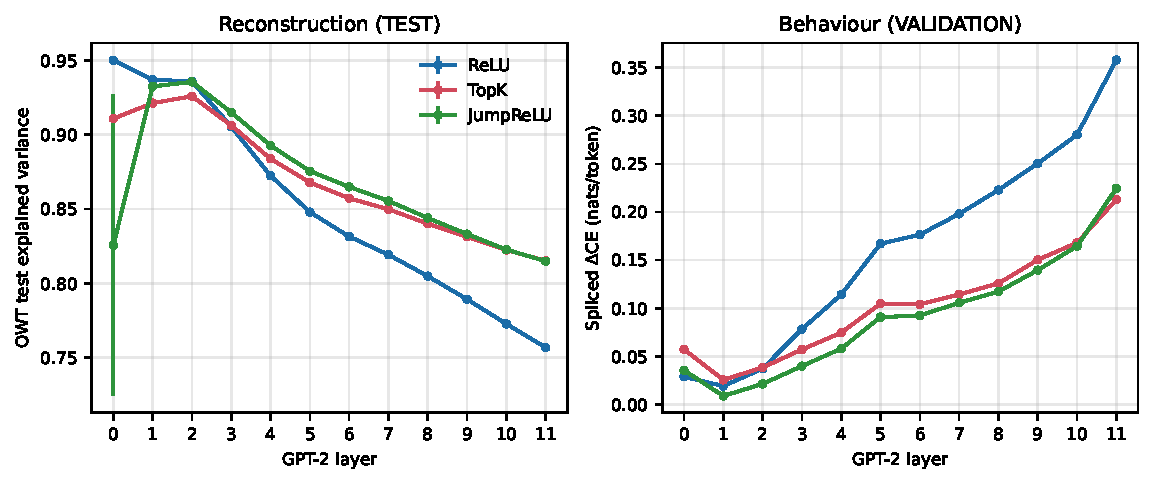
\includegraphics[width=\linewidth]{fig_reconstruction_behaviour}
  \caption{Left: OWT test explained variance by layer (\evlabel{test}; error bars: seed sd). Right: spliced
  next-token cross-entropy increase (\evlabel{validation}). Sources: Tables~\ref{tab:recon} and~\ref{tab:splice}.}
  \label{fig:recon}
\end{figure}

\pending{E1 (TopK trained at several $k$ to match task-level L0) and E2 (public \texttt{gpt2-small-res-jb}
reference; not matched in width, data or L0).}
